% Options for packages loaded elsewhere
% Options for packages loaded elsewhere
\PassOptionsToPackage{unicode}{hyperref}
\PassOptionsToPackage{hyphens}{url}
\PassOptionsToPackage{dvipsnames,svgnames,x11names}{xcolor}
%
\documentclass[
  letterpaper,
  DIV=11,
  numbers=noendperiod]{scrartcl}
\usepackage{xcolor}
\usepackage{amsmath,amssymb}
\setcounter{secnumdepth}{5}
\usepackage{iftex}
\ifPDFTeX
  \usepackage[T1]{fontenc}
  \usepackage[utf8]{inputenc}
  \usepackage{textcomp} % provide euro and other symbols
\else % if luatex or xetex
  \usepackage{unicode-math} % this also loads fontspec
  \defaultfontfeatures{Scale=MatchLowercase}
  \defaultfontfeatures[\rmfamily]{Ligatures=TeX,Scale=1}
\fi
\usepackage{lmodern}
\ifPDFTeX\else
  % xetex/luatex font selection
\fi
% Use upquote if available, for straight quotes in verbatim environments
\IfFileExists{upquote.sty}{\usepackage{upquote}}{}
\IfFileExists{microtype.sty}{% use microtype if available
  \usepackage[]{microtype}
  \UseMicrotypeSet[protrusion]{basicmath} % disable protrusion for tt fonts
}{}
\makeatletter
\@ifundefined{KOMAClassName}{% if non-KOMA class
  \IfFileExists{parskip.sty}{%
    \usepackage{parskip}
  }{% else
    \setlength{\parindent}{0pt}
    \setlength{\parskip}{6pt plus 2pt minus 1pt}}
}{% if KOMA class
  \KOMAoptions{parskip=half}}
\makeatother
% Make \paragraph and \subparagraph free-standing
\makeatletter
\ifx\paragraph\undefined\else
  \let\oldparagraph\paragraph
  \renewcommand{\paragraph}{
    \@ifstar
      \xxxParagraphStar
      \xxxParagraphNoStar
  }
  \newcommand{\xxxParagraphStar}[1]{\oldparagraph*{#1}\mbox{}}
  \newcommand{\xxxParagraphNoStar}[1]{\oldparagraph{#1}\mbox{}}
\fi
\ifx\subparagraph\undefined\else
  \let\oldsubparagraph\subparagraph
  \renewcommand{\subparagraph}{
    \@ifstar
      \xxxSubParagraphStar
      \xxxSubParagraphNoStar
  }
  \newcommand{\xxxSubParagraphStar}[1]{\oldsubparagraph*{#1}\mbox{}}
  \newcommand{\xxxSubParagraphNoStar}[1]{\oldsubparagraph{#1}\mbox{}}
\fi
\makeatother


\usepackage{longtable,booktabs,array}
\newcounter{none} % for unnumbered tables
\usepackage{calc} % for calculating minipage widths
% Correct order of tables after \paragraph or \subparagraph
\usepackage{etoolbox}
\makeatletter
\patchcmd\longtable{\par}{\if@noskipsec\mbox{}\fi\par}{}{}
\makeatother
% Allow footnotes in longtable head/foot
\IfFileExists{footnotehyper.sty}{\usepackage{footnotehyper}}{\usepackage{footnote}}
\makesavenoteenv{longtable}
\usepackage{graphicx}
\makeatletter
\newsavebox\pandoc@box
\newcommand*\pandocbounded[1]{% scales image to fit in text height/width
  \sbox\pandoc@box{#1}%
  \Gscale@div\@tempa{\textheight}{\dimexpr\ht\pandoc@box+\dp\pandoc@box\relax}%
  \Gscale@div\@tempb{\linewidth}{\wd\pandoc@box}%
  \ifdim\@tempb\p@<\@tempa\p@\let\@tempa\@tempb\fi% select the smaller of both
  \ifdim\@tempa\p@<\p@\scalebox{\@tempa}{\usebox\pandoc@box}%
  \else\usebox{\pandoc@box}%
  \fi%
}
% Set default figure placement to htbp
\def\fps@figure{htbp}
\makeatother

\ifLuaTeX
  \usepackage{luacolor}
  \usepackage[soul]{lua-ul}
\else
  \usepackage{soul}
\fi




\setlength{\emergencystretch}{3em} % prevent overfull lines

\providecommand{\tightlist}{%
  \setlength{\itemsep}{0pt}\setlength{\parskip}{0pt}}



 


\KOMAoption{captions}{tableheading}
\usepackage{pdfpages}
\usepackage{graphicx}
\usepackage{eso-pic}
\usepackage{tocloft}
\renewcommand{\cfttoctitlefont}{\Huge\bfseries}
\renewcommand{\cftaftertoctitle}{\vspace{1cm}}
\renewcommand{\cftsecfont}{\fontsize{13pt}{15pt}\selectfont\bfseries}
\renewcommand{\cftsecpagefont}{\fontsize{13pt}{15pt}\selectfont\bfseries}
\setlength{\cftbeforesecskip}{18pt}
\setlength{\cftsecindent}{0pt}
\renewcommand{\cftsubsecfont}{\large}
\renewcommand{\cftsubsecpagefont}{\large}
\setlength{\cftbeforesubsecskip}{12pt}
\setlength{\cftsubsecindent}{1.5em}
\renewcommand{\cftsubsubsecfont}{\normalsize}
\renewcommand{\cftsubsubsecpagefont}{\normalsize}
\setlength{\cftbeforesubsubsecskip}{8pt}
\setlength{\cftsubsubsecindent}{3em}
\makeatletter
\@ifpackageloaded{caption}{}{\usepackage{caption}}
\AtBeginDocument{%
\ifdefined\contentsname
  \renewcommand*\contentsname{Table of contents}
\else
  \newcommand\contentsname{Table of contents}
\fi
\ifdefined\listfigurename
  \renewcommand*\listfigurename{List of Figures}
\else
  \newcommand\listfigurename{List of Figures}
\fi
\ifdefined\listtablename
  \renewcommand*\listtablename{List of Tables}
\else
  \newcommand\listtablename{List of Tables}
\fi
\ifdefined\figurename
  \renewcommand*\figurename{Figure}
\else
  \newcommand\figurename{Figure}
\fi
\ifdefined\tablename
  \renewcommand*\tablename{Table}
\else
  \newcommand\tablename{Table}
\fi
}
\@ifpackageloaded{float}{}{\usepackage{float}}
\floatstyle{ruled}
\@ifundefined{c@chapter}{\newfloat{codelisting}{h}{lop}}{\newfloat{codelisting}{h}{lop}[chapter]}
\floatname{codelisting}{Listing}
\newcommand*\listoflistings{\listof{codelisting}{List of Listings}}
\makeatother
\makeatletter
\makeatother
\makeatletter
\@ifpackageloaded{caption}{}{\usepackage{caption}}
\@ifpackageloaded{subcaption}{}{\usepackage{subcaption}}
\makeatother
\usepackage{bookmark}
\IfFileExists{xurl.sty}{\usepackage{xurl}}{} % add URL line breaks if available
\urlstyle{same}
% fallback for those not using the hyperref driver hyperxmp:
\makeatletter
\@ifundefined{xmpquote}{\newcommand{\xmpquote}[1]{#1}}{}
\makeatother
\hypersetup{
  colorlinks=true,
  linkcolor={blue},
  filecolor={Maroon},
  citecolor={Blue},
  urlcolor={Blue},
  pdfcreator={LaTeX via pandoc}}


\author{}
\date{}
\begin{document}

\renewcommand*\contentsname{Table des matières}
{
\setcounter{tocdepth}{3}
\tableofcontents
}

\newpage

\section{Introduction}\label{introduction}

Depuis plusieurs années, le numérique a profondément transformé la
manière dont nous consommons et partageons nos loisirs culturels. Le
cinéma dispose de Letterboxd, la musique de Last.fm : des plateformes
communautaires qui permettent à chacun de garder une trace de ses
découvertes, de les noter et d'échanger avec d'autres passionnés. La
lecture, pourtant, reste étonnamment mal servie sur ce plan. Le
principal service existant, Goodreads, appartient à Amazon, ce qui pose
des questions en matière d'indépendance éditoriale et d'exploitation des
données personnelles des lecteurs.

C'est de ce constat qu'est né le projet Ex-Libris : une application de
suivi de lecture pensée comme un véritable réseau social pour les
lecteurs. L'objectif n'est pas de reconstruire un catalogue de livres,
un travail déjà accompli et maintenu par la plateforme collaborative
Open Library, qui référence plusieurs millions d'ouvrages en accès
libre. Ce qu'Open Library ne propose pas, en revanche, c'est la
dimension humaine de la lecture : qui a lu quel livre, quand, avec quel
avis, et quelles recommandations peuvent en être tirées. C'est
précisément cette couche que notre application vient ajouter.

Concrètement, Ex-Libris doit permettre à un utilisateur de créer un
compte, de rechercher un livre et d'en consulter la fiche détaillée, de
l'ajouter à sa bibliothèque personnelle avec un statut de lecture, de le
noter et d'en rédiger une critique. Au-delà de cette gestion
individuelle, l'application intègre une dimension sociale : chaque
utilisateur peut consulter le profil d'un autre lecteur, s'abonner à son
activité, et bénéficier d'un système de recommandation construit à
partir des affinités entre utilisateurs.

D'un point de vue technique, le projet repose sur une API REST
développée avec FastAPI, exploitant les données de l'API publique Open
Library et s'appuyant sur une base de données PostgreSQL pour la
persistance des données propres à notre application. Le langage retenu
est Python, dans une logique de programmation orientée objet.

Ce dossier présente dans un premier temps le cahier des charges du
projet, les choix et arbitrages qui ont guidé nos réflexions, ainsi que
l'organisation retenue au sein de notre équipe. Il détaille ensuite le
modèle de conception élaboré pour répondre à ces besoins, à travers les
différents diagrammes UML réalisés.

\newpage

\section{Cahier des Charges}\label{cahier-des-charges}

Ce cahier des charges exprime le besoin initial auquel notre application
doit répondre : une application de suivi de lecture combinant la
richesse du catalogue d'Open Library à une véritable dimension sociale
entre lecteurs. Sur cette base, notre travail a consisté à reformuler ce
besoin, à en préciser le périmètre exact, et à définir les
fonctionnalités attendues ainsi que les contraintes techniques qui en
découlent, notamment celles liées à l'exploitation d'une source de
données externe.

\subsection{Présentation d'Open
Library}\label{pruxe9sentation-dopen-library}

\begin{flushright}
\vspace{-1cm}
\end{flushright}

Notre application repose entièrement sur les données fournies par Open
Library, une base collaborative et gratuite qui référence plusieurs
millions d'ouvrages. Il s'agit d'une API web : on l'interroge en
construisant des adresses (URLs) spécifiques, et elle nous renvoie les
données demandées au format JSON.
\#
\includegraphics[width=0.15\textwidth]{OL_logo.png}

\begin{center}

\includegraphics[width=0.8\textwidth]{API1.png}
\end{center}

Pour bien comprendre comment exploiter ces données, il est essentiel de
saisir la façon dont Open Library organise ses informations. La base
distingue en réalité trois notions différentes qui, dans le langage
courant, sont toutes désignées par le mot ``livre'' :

\begin{itemize}
\tightlist
\item
  L'auteur (Author) : la personne ayant écrit l'œuvre.
\item
  L'œuvre (Work) : il s'agit de l'idée générale du livre, indépendamment
  de toute édition particulière. C'est à ce niveau que l'on trouve par
  exemple le titre, un résumé, ou les grands thèmes abordés.
\item
  L'édition (Edition) : il s'agit d'une publication précise et
  matérielle de cette œuvre, par exemple une édition Harcourt de 1971.
  Une même œuvre peut avoir des centaines d'éditions différentes
  (traductions, rééditions, formats poche\ldots).
\end{itemize}

Dans notre base de données, nous avons fait le choix de conserver, pour
chaque œuvre, l'ensemble de ses éditions, afin d'offrir aux utilisateurs
une réelle variété de choix (langue, édition, format) lorsqu'ils
ajoutent un livre à leur bibliothèque. Nous détaillerons la façon dont
nous avons stocké et traité ces données dans la suite de ce dossier
d'analyse, lors de la conception de la maquette.

Nous avons également constaté que certaines données présentes dans Open
Library manquent de cohérence, notamment les thèmes et genres associés
aux œuvres (champ subjects), qui sont rédigés en texte libre et
mélangent parfois de véritables genres littéraires avec de simples
mots-clés. Cette hétérogénéité a directement motivé l'une de nos
réflexions pour la fonctionnalité de normalisation des genres, qui vise
à proposer une classification plus cohérente et plus facilement
exploitable pour la recherche par genre.

\begin{center}

\begin{minipage}{0.45\textwidth}
\centering

\includegraphics[width=\textwidth]{work.png}
\end{minipage}
\hfill
\begin{minipage}{0.45\textwidth}
\centering

\includegraphics[width=\textwidth]{edition.png}
\end{minipage}

\vspace{0.3cm}


\includegraphics[width=0.6\textwidth]{auteur.png}

\end{center}

\newpage

\subsection{Diagramme de cas
d'utilisation}\label{diagramme-de-cas-dutilisation}

\begin{center}

\includegraphics[width=0.62\textwidth]{cas_usage.png}

Figure 11 – Diagramme de cas d'utilisation
\end{center}

\newpage

\subsection{Diagramme d'activité}\label{diagramme-dactivituxe9}

\newpage

\section{Organisation du projet}\label{organisation-du-projet}

\subsection{Organisation du groupe}\label{organisation-du-groupe}

Dès le début du projet, nous avons désigné Anne-Camille Tampet comme
cheffe de projet et Cécile Locatelli comme leader technique, en
veillant, conformément aux conseils donnés en début de projet à ne pas
cumuler ces deux rôles sur une même personne.

Pour communiquer, nous avons créé un groupe sur Teams, sur lequel chacun
peut partager ses avancées, poser une question ou signaler un point de
blocage dès que le besoin s'en fait sentir. C'est notre principal canal
d'échange, sur lequel nous discutons régulièrement. En parallèle, nous
avons mis en place un dépôt partagé sur GitHub, accessible à tous les
membres du groupe, qui nous sert à centraliser et à distribuer
l'ensemble des fichiers importants du projet.

Concernant la répartition du travail, notre organisation a surtout été
pensée pour cette première phase d'analyse. Chaque membre du groupe
s'est vu confier la réalisation d'un diagramme ou d'une partie
spécifique du dossier, de façon à ce que chacun puisse s'investir
concrètement dans la réflexion et la conception du projet. Cette
répartition individuelle ne nous a cependant pas empêchés de travailler
de façon très collective. Nous avons pris l'habitude de nous retrouver
au minimum deux fois par semaine pour faire le point ensemble. Ces
moments nous permettaient de relire et de discuter les diagrammes
réalisés par chacun, de nous assurer que tout le monde comprenait bien
les choix faits par les autres et de les faire évoluer si nécessaire.
Cette phase de discussion collective a été particulièrement importante
en tout début de projet. Elle nous a permis de poser une base commune
solide et de nous assurer que tout le monde partageait la même vision de
l'application avant d'avancer plus en détail sur la partie codage.

\begin{center}

\includegraphics[width=0.62\textwidth]{git.png}

Figure 11 – Dépot Github
\end{center}

\subsection{Diagramme de Gantt}\label{diagramme-de-gantt}

\begin{center}

\includegraphics[width=0.8\textwidth]{Gantt.png}

Figure 11 – Diagramme de Gantt
\end{center}

Notre planning se découpe en deux grandes phases. D'abord la phase
d'analyse, de fin août à fin septembre : nous commençons par étudier
l'API Open Library, puis nous réalisons l'ensemble de la modélisation
UML afin de bien comprendre comment notre application va s'articuler et
comment la construire.

Une fois cette base posée, nous passons à la phase de code, d'octobre à
début novembre. Nous avons choisi de développer les fonctionnalités par
ordre de difficulté croissante : d'abord les classes de base, puis
l'authentification et la recherche de livres (F1-F2), la bibliothèque
avec les statuts de lecture (F3), les critiques (F4), et enfin notre
fonctionnalité F5 (les recommandations), qui nécessitera davantage de
temps du fait de sa complexité. Les tests unitaires et le frontend
interviendront en dernier, le frontend n'étant pas prioritaire, sera
développé uniquement s'il nous reste du temps.

\newpage

\section{Maquette de l'application}\label{maquette-de-lapplication}

\subsection{Diagrammes de base de
données}\label{diagrammes-de-base-de-donnuxe9es}

La conception de la base de données de l'application repose sur la
séparation entre les informations bibliographiques des livres et les
données propres aux utilisateurs de l'application. Les informations
générales concernant les livres sont récupérées à partir de l'API Open
Library. Il n'est donc pas nécessaire de reconstruire localement un
catalogue complet de livres. La base de données de l'application est
principalement destinée à conserver les utilisateurs ainsi que les
différentes interactions qu'ils peuvent avoir avec les livres :
lectures, critiques et appréciations. Elle permet également de gérer les
relations entre les utilisateurs à travers le système d'abonnement.

La base est composée de six tables : \texttt{Utilisateur},
\texttt{Livre}, \texttt{Lecture}, \texttt{Critique}, \texttt{Abonnement}
et \texttt{Like}.

\begin{center}

\includegraphics[width=0.8\textwidth]{BDD.png}

Figure 11 – Diagramme de base de données
\end{center}

\subsubsection{Table Utilisateur}\label{table-utilisateur}

La table \textbf{\texttt{Utilisateur}} représente les personnes
utilisant l'application. Elle contient un identifiant unique
\texttt{id\_user}, de type \texttt{SERIAL}, qui constitue la clé
primaire. Les autres attributs sont \texttt{pseudo}, \texttt{email},
\texttt{password\_hash} et \texttt{bio}, qui correspondent
respectivement au pseudonyme, à l'adresse électronique, au mot de passe
sous forme de hash et à la biographie de l'utilisateur.

Cette table constitue une entité centrale de la base puisque les
fonctionnalités personnalisées de l'application, telles que la gestion
des lectures, la publication de critiques et les abonnements, sont
associées à un utilisateur.

\subsubsection{Table Livre}\label{table-livre}

La table \textbf{\texttt{Livre}} représente les ouvrages enregistrés
dans l'application. Elle possède un identifiant unique
\texttt{id\_livre}, de type \texttt{SERIAL}, qui constitue la clé
primaire de la table. L'attribut \texttt{id\_work}, de type
\texttt{VARCHAR}, correspond à l'identifiant de l'œuvre fourni par Open
Library. Il permet d'identifier l'ouvrage dans le catalogue Open Library
et d'établir le lien entre l'enregistrement présent dans notre base et
les informations bibliographiques fournies par l'API.

Bien que \texttt{id\_work} permette déjà d'identifier une œuvre dans
Open Library, nous avons choisi de définir notre propre clé primaire
\texttt{id\_livre}. Cela permet à notre base de données de disposer d'un
identifiant interne indépendant de l'API externe. Ainsi, l'organisation
et l'identification des livres dans notre base ne dépendent pas
directement du fonctionnement ou de l'évolution des identifiants fournis
par Open Library. \texttt{id\_work} est alors utilisé comme référence
vers Open Library, tandis que \texttt{id\_livre} constitue la référence
interne utilisée par les autres tables de notre base, notamment
\texttt{Lecture}.

Les attributs \texttt{titre} et \texttt{auteurs} permettent de conserver
localement les principales informations bibliographiques nécessaires à
l'application. Le fait de stocker ces informations dans notre base
permet de les consulter rapidement sans devoir effectuer
systématiquement une nouvelle requête auprès d'Open Library. Cela permet
également de limiter le nombre d'appels à l'API, qui impose une
limitation du nombre de requêtes par seconde.

Les informations bibliographiques supplémentaires qui ne sont pas
nécessaires au fonctionnement immédiat de l'application peuvent, quant à
elles, être récupérées directement auprès d'Open Library lorsque cela
est nécessaire. La base locale conserve donc uniquement les informations
utiles de manière récurrente, tandis que l'API reste la source des
informations bibliographiques complémentaires.

\subsubsection{Table Lecture}\label{table-lecture}

La table \textbf{\texttt{Lecture}} représente les interactions de
lecture entre les utilisateurs et les livres. Elle possède un
identifiant unique \texttt{id\_lecture}, de type \texttt{SERIAL}, qui
constitue sa clé primaire.

Elle contient deux clés étrangères :

\begin{itemize}
\tightlist
\item
  \texttt{id\_user}, de type \texttt{INT}, qui fait référence à
  \texttt{Utilisateur(id\_user)}.
\item
  \texttt{id\_livre}, de type \texttt{INT}, qui fait référence à
  \texttt{Livre(id\_livre)}.
\end{itemize}

Ces deux attributs permettent d'identifier l'utilisateur concerné et le
livre auquel se rapporte la lecture. La table contient également
\texttt{statut}, \texttt{date\_ajout}, \texttt{date\_lu} et
\texttt{note}.

L'attribut \texttt{statut} permet de représenter l'état de lecture d'un
livre, par exemple : pas commencé, en cours, lu ou abandonné. L'attribut
\texttt{date\_ajout} correspond à la date à laquelle le livre a été
ajouté à la bibliothèque de l'utilisateur, tandis que \texttt{date\_lu}
permet d'enregistrer la date de fin de lecture. L'attribut
\texttt{note}, de type \texttt{INT}, permet de conserver une note
attribuée au livre après l'avoir lu.

Le recours à cette table permet de représenter une relation
plusieurs-à-plusieurs entre les utilisateurs et les livres. En effet, un
utilisateur peut enregistrer plusieurs lectures et un même livre peut
être enregistré par plusieurs utilisateurs. La table \texttt{Lecture}
permet donc de matérialiser cette relation tout en conservant les
informations propres à chaque interaction.

\subsubsection{Table Critique}\label{table-critique}

La table \textbf{\texttt{Critique}} permet de gérer les avis publiés sur
les livres. Elle possède un identifiant unique \texttt{id\_critique}, de
type \texttt{INT}, qui constitue sa clé primaire.

L'attribut \texttt{id\_lecture}, de type \texttt{INT}, constitue une clé
étrangère faisant référence à \texttt{Lecture(id\_lecture)}. Il permet
de rattacher chaque critique à une lecture enregistrée dans la base de
données. Les autres attributs sont \texttt{texte}, qui contient le
contenu de la critique, et \texttt{date\_publication}, qui correspond à
la date de publication de l'avis.

La critique est ainsi associée indirectement à un utilisateur et à un
livre à travers la table \texttt{Lecture}. Ce choix permet de rattacher
une critique à une interaction de lecture précise plutôt que de la
relier directement à un livre.

D'après le diagramme, une lecture peut recevoir au maximum une critique
(\texttt{0..1}). Une critique est obligatoirement associée à une seule
lecture. Cette cardinalité traduit le choix de conception selon lequel
une lecture enregistrée peut être accompagnée d'une critique unique.

L'identifiant propre à la critique est également nécessaire pour la
gestion des appréciations. Une critique constitue en effet un objet
identifié sur lequel les utilisateurs peuvent interagir.

\subsubsection{Table Like}\label{table-like}

La table \textbf{\texttt{Like}} représente les appréciations associées
aux critiques. Elle contient deux clés étrangères :

\begin{itemize}
\tightlist
\item
  \texttt{id\_user}, qui fait référence à
  \texttt{Utilisateur(id\_user)}.
\item
  \texttt{id\_critique}, qui fait référence à
  \texttt{Critique(id\_critique)}.
\end{itemize}

Ces deux attributs constituent ensemble la clé primaire composite de la
table. Cette clé permet d'identifier de manière unique l'association
entre un utilisateur et une critique, et d'éviter qu'un même utilisateur
enregistre plusieurs fois la même appréciation pour une critique donnée.

La table contient également \texttt{date\_like}, de type \texttt{DATE},
qui permet de conserver la date de l'appréciation, ainsi que
\texttt{aime}, de type \texttt{BOOL}, qui indique la nature de
l'interaction. La valeur \texttt{TRUE} peut représenter un « j'aime » et
la valeur \texttt{FALSE} un « je n'aime pas ».

La table \texttt{Like} matérialise ainsi une relation
plusieurs-à-plusieurs entre les utilisateurs et les critiques : un
utilisateur peut apprécier plusieurs critiques et une même critique peut
être appréciée par plusieurs utilisateurs.

\subsubsection{Table Abonnement}\label{table-abonnement}

Enfin, la table \textbf{\texttt{Abonnement}} permet de représenter les
relations entre les utilisateurs. Elle met en relation deux instances de
la même entité \texttt{Utilisateur}, correspondant à deux rôles
différents.

Elle contient deux clés étrangères :

\begin{itemize}
\tightlist
\item
  \texttt{id\_follower}, de type \texttt{SERIAL}, qui fait référence à
  \texttt{Utilisateur(id\_user)} et désigne l'utilisateur qui s'abonne.
\item
  \texttt{id\_followed}, de type \texttt{INT}, qui fait référence à
  \texttt{Utilisateur(id\_user)} et désigne l'utilisateur suivi.
\end{itemize}

Ces deux attributs constituent ensemble la clé primaire composite de la
table. La date de l'abonnement est conservée dans l'attribut
\texttt{date\_abonnement}.

\subsection{Diagramme de classes}\label{diagramme-de-classes}

\subsubsection{Classes Business Object}\label{classes-business-object}

\begin{center}

\includegraphics[width=0.8\textwidth]{Buissiness_object.png}

Figure 11 – Diagramme de classe : Business Object
\end{center}

\subsubsection{Classes DAO}\label{classes-dao}

\subsubsection{Classes Service}\label{classes-service}

\newpage

\subsection{Diagrammes de séquence}\label{diagrammes-de-suxe9quence}

Les diagrammes de séquence suivant permettent de détailler la
chronologie des échanges entre les différents composants de notre
architecture (Utilisateur, Front End, Back End, DAO, API externe) pour
trois fonctionnalités de l'application : la suppression d'une fiche de
lecture, la sélection d'un livre et la demande de recommandations
personnalisées.

\begin{center}
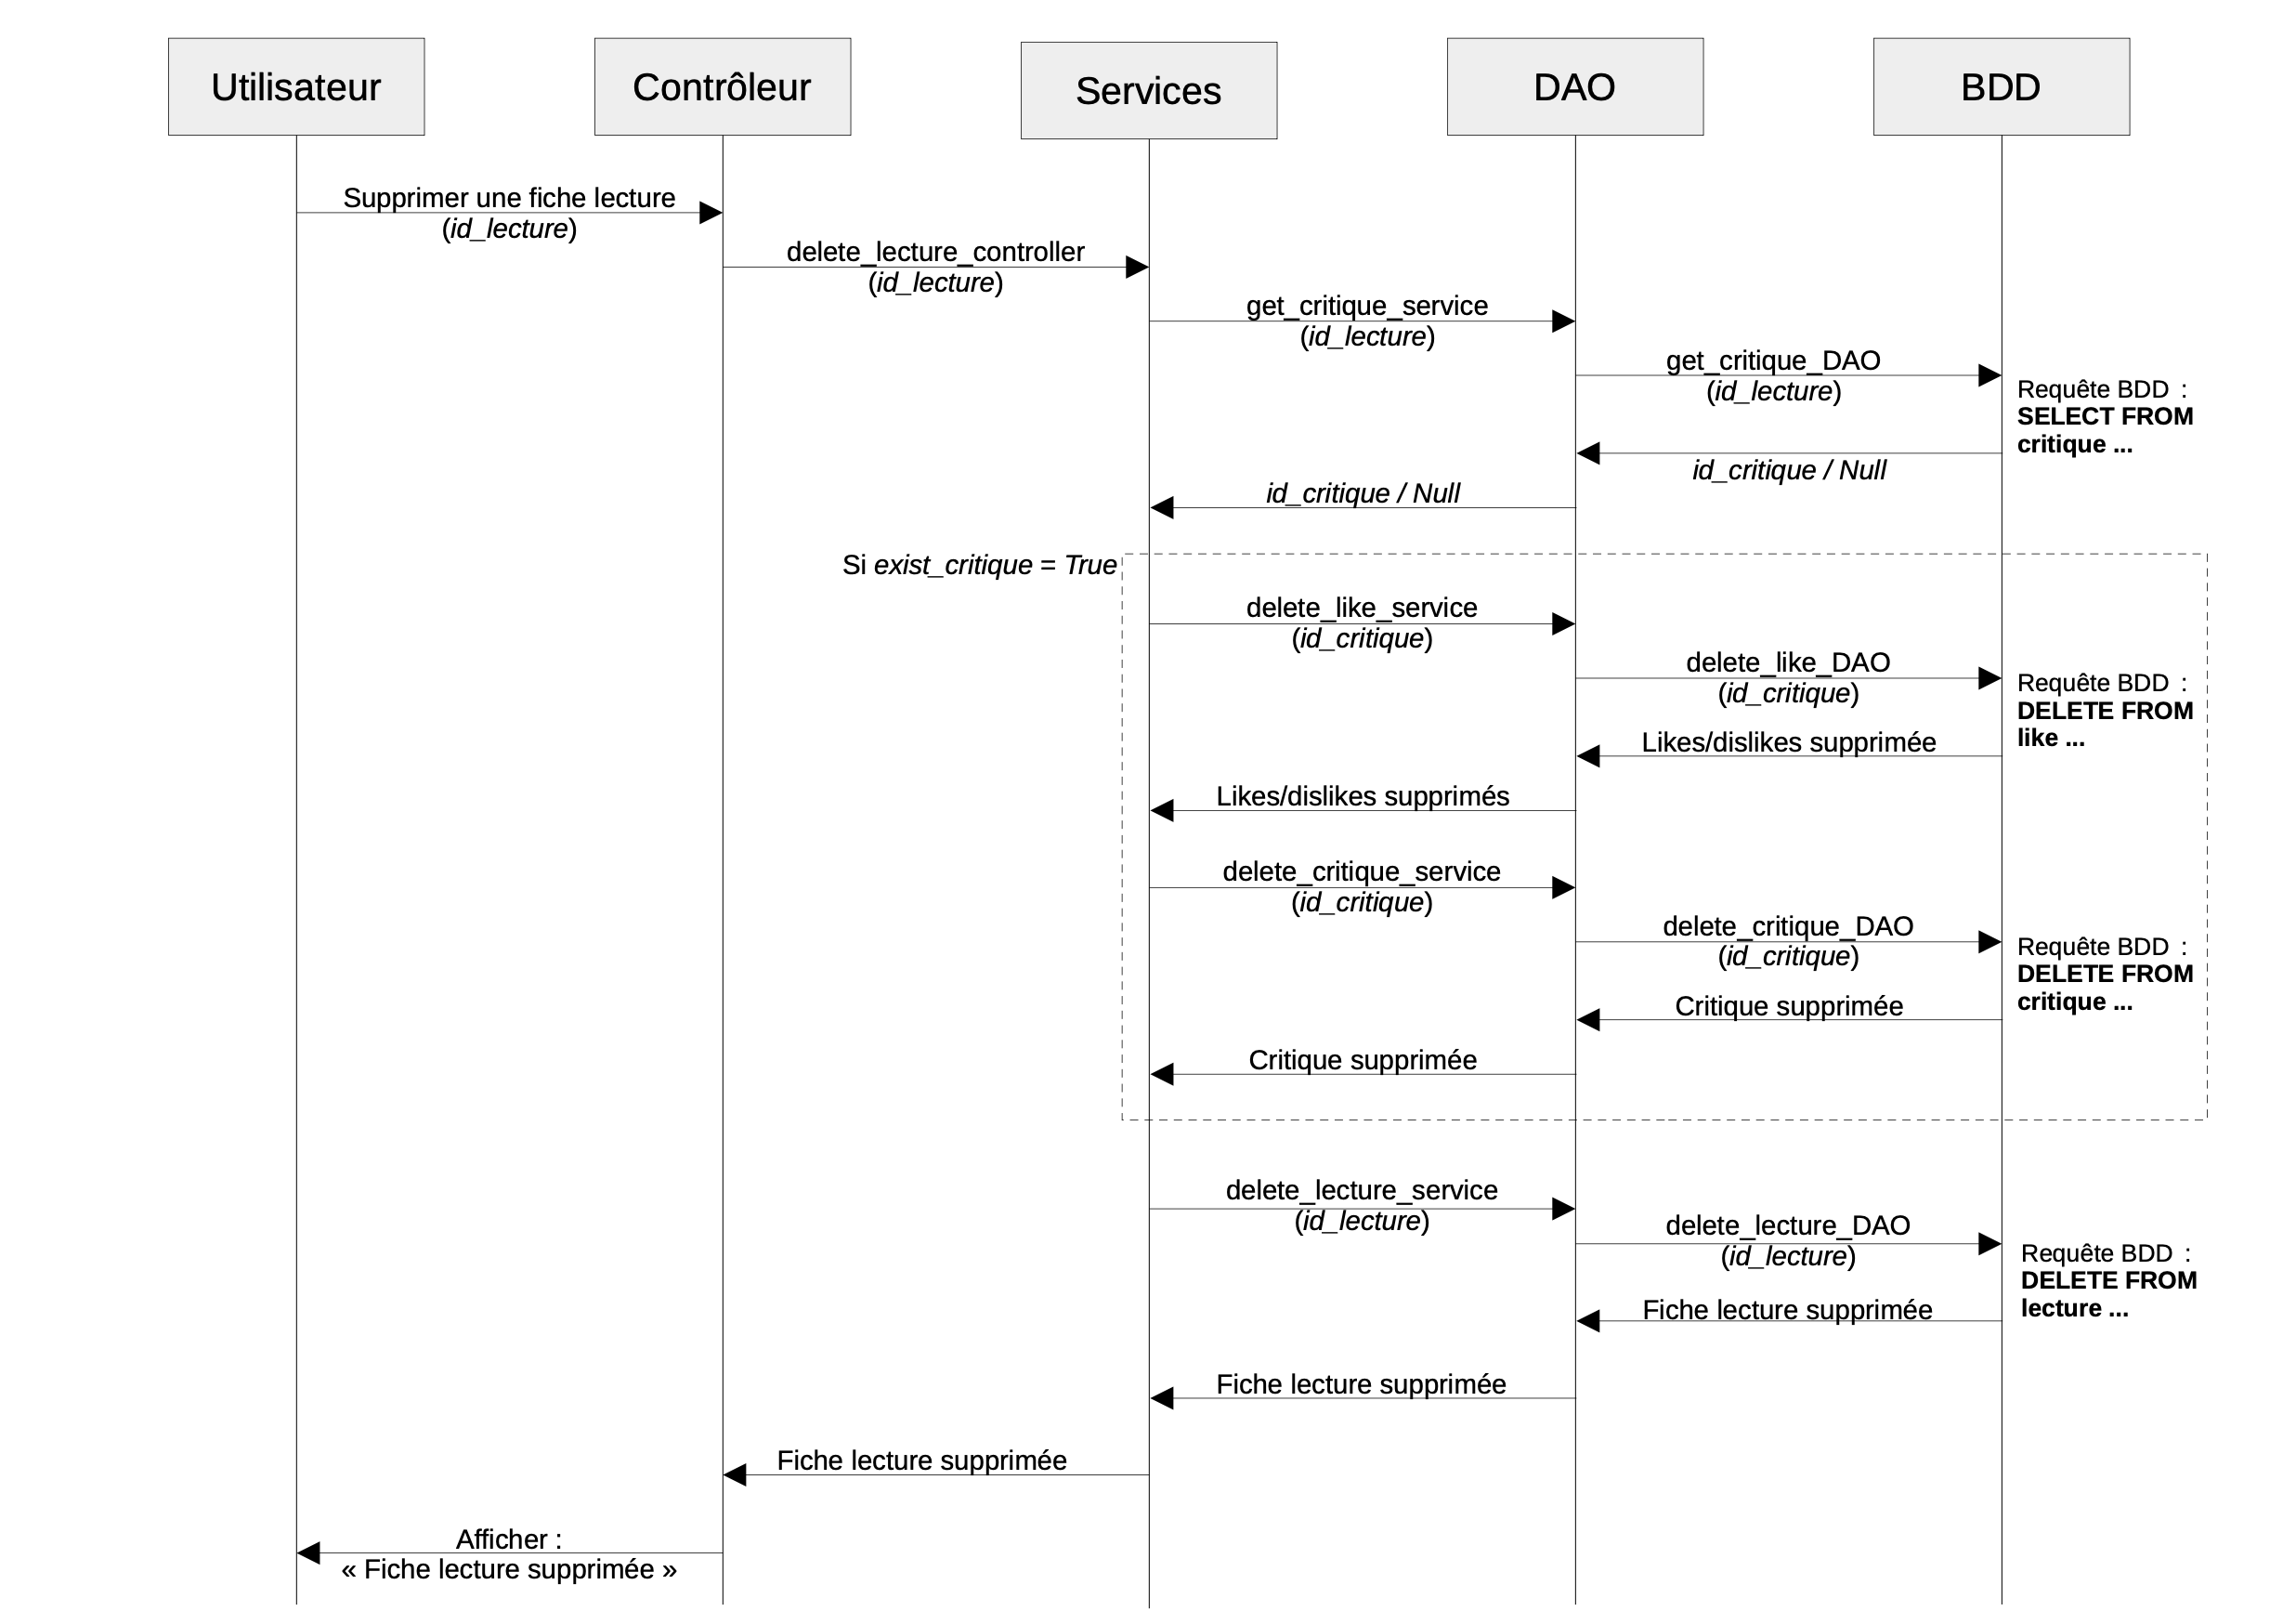
\includegraphics[width=0.8\textwidth]{Diagramme_Séquence_Suppression-fiche-lecture_page-0001.jpg}

Figure 11 – Diagramme de séquence : supprimer une fiche de lecture
\end{center}

Le but de cette séquence est de supprimer une fiche lecture pour un
utilisateur.

Celui-ci a créé auparavant une fiche lecture : il a enregistré un livre
avec des informations (statut du livre, note, etc., il a éventuellement
ajouté une critique associée). Il souhaite aujourd'hui la supprimer.

Il se situe au départ sur la fiche lecture considérée, et clique sur un
bouton « Supprimer la fiche lecture ».

L'information, avec l'\texttt{id\_lecture} (l'identifiant de la fiche
lecture) est réceptionnée par le \textbf{Contrôleur}, qui la transmet au
\textbf{Service}, qui envoie des requêtes au \textbf{DAO}.

Dans un premier temps, le \textbf{Service} va rechercher dans la base de
données l'existence éventuelle d'une \texttt{critique} associée à cette
lecture. Si une \texttt{critique} est trouvée, alors celle-ci sera
supprimée, ainsi que d'éventuels likes/dislikes associés.

Ensuite, la fiche lecture est supprimée de la table de données «
\texttt{lecture} ».

À la fin de toutes ces opérations, le \textbf{Service} transmet au
\textbf{Contrôleur} l'information que la fiche a bien été supprimée,
celui-ci affiche à l'écran de l'utilisateur « La fiche lecture a bien
été supprimée ».

\begin{center}
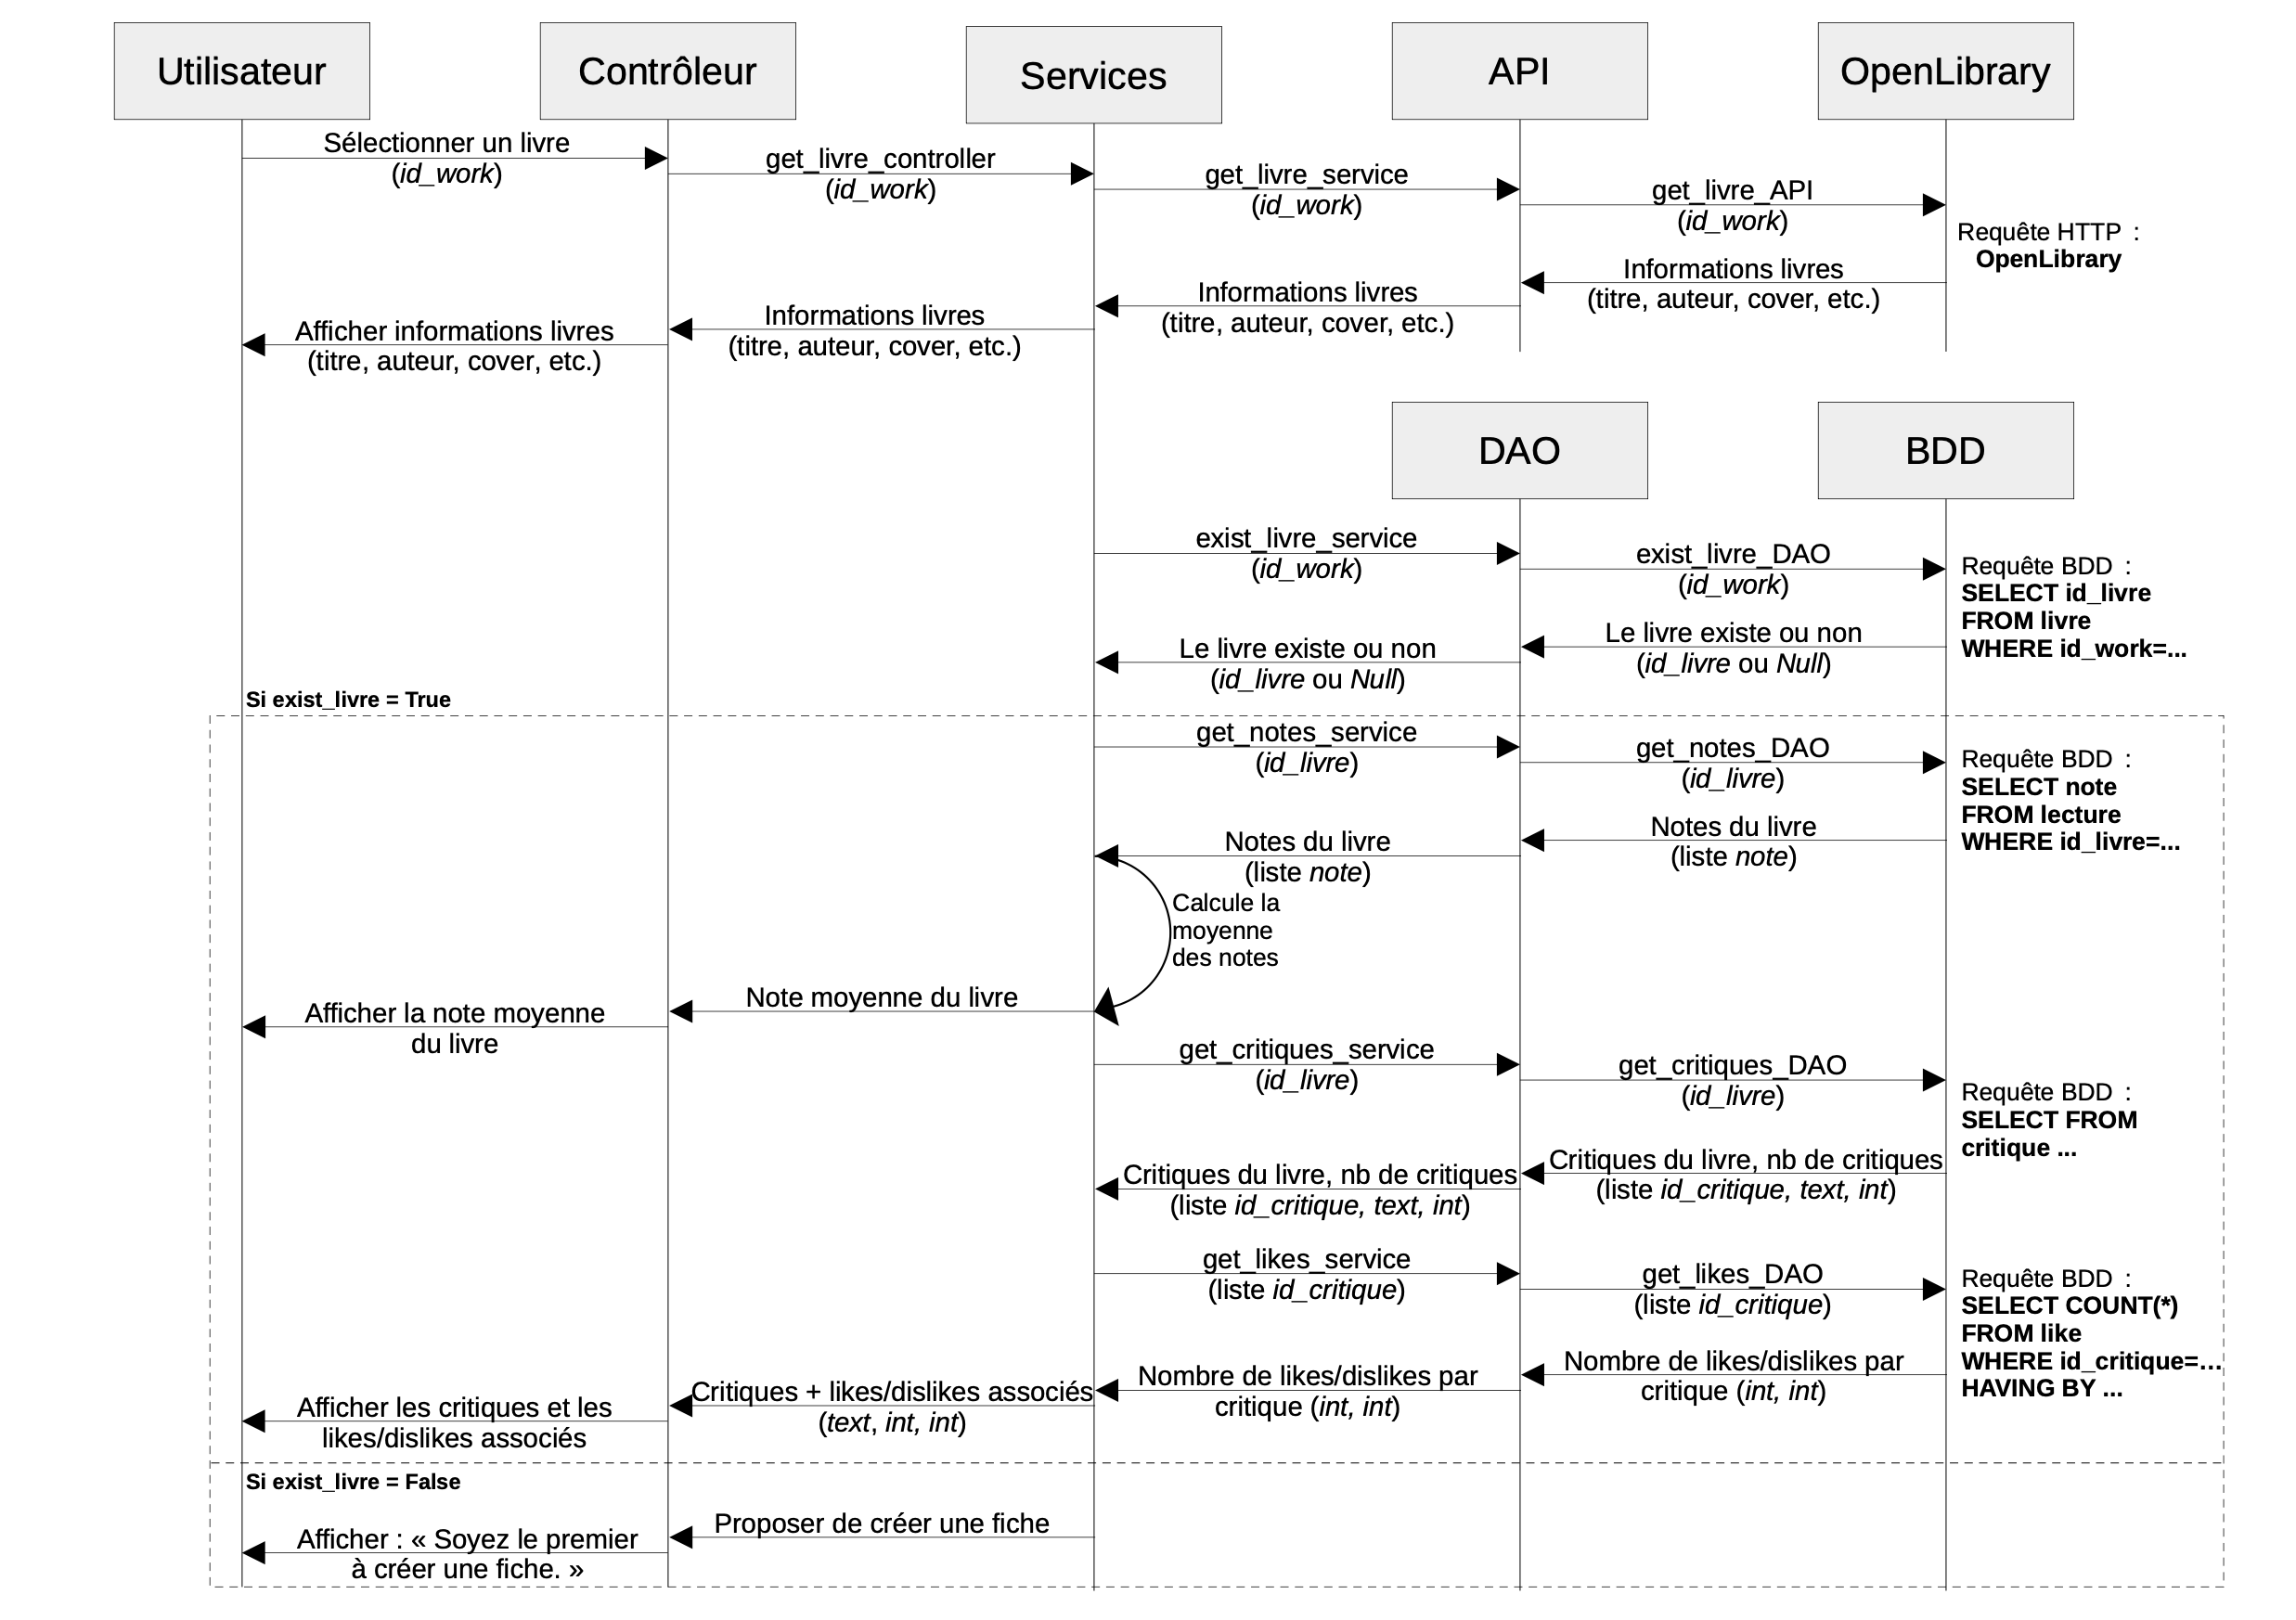
\includegraphics[width=0.8\textwidth]{Diagramme_Séquence_Sélectionner-livre_page-0001.jpg}

Figure 11 – Diagramme de séquence : sélectionner un livre
\end{center}

Le but de cette séquence est d'afficher toutes les informations
disponibles sur un livre sélectionné par un utilisateur.

Celui-ci a par exemple effectué une recherche, a obtenu une liste de
livres (correspondant à une liste de \texttt{id\_work}, les identifiants
stockés par \textbf{OpenLibrary}), il choisit l'un d'entre eux pour en
afficher toutes les informations.

La première étape est de récupérer les informations fournies par
\textbf{OpenLibrary} sur ce livre : le \textbf{Contrôleur} va
transmettre au \textbf{Service} l'\texttt{id\_work} considéré, pour
utiliser l'\textbf{API} qui va effectuer une requête au niveau
d'\textbf{OpenLibrary}.

De cette requête, on va récupérer les informations pertinentes contenues
dans \textbf{OpenLibrary} (titre, auteur, date, cover, etc. -- la liste
précise reste à définir).

Ensuite, il s'agit de fournir les informations propres à notre
application Ex-Libris.

Pour cela, le \textbf{Service} va transmettre l'\texttt{id\_work} au
\textbf{DAO}, qui va rechercher dans la base de données si un livre a
déjà été enregistré associé à celui-ci. Si oui, le \textbf{DAO}
remontera au \textbf{Service} un \texttt{id\_livre} correspondant.

Sinon, il lui proposera d'être le premier à créer une fiche lecture.

À partir de cet \texttt{id\_livre}, le \textbf{Service} va demander au
\textbf{DAO} de récupérer toutes les notes mises par les utilisateurs à
ce livre, pour ensuite en faire la moyenne.

Il va ensuite rechercher les critiques (\texttt{critique}) associées à
ce livre, leur nombre, et les likes/dislikes (\texttt{like}) associés.
Si de nombreuses critiques ont été rédigées sur ce livre, il sera
possible de n'en choisir que quelques-unes (par exemple, celles avec le
plus grand nombre de likes), même si cela n'apparaît pas dans le
diagramme pour éviter une surcharge visuelle.

Le \textbf{Service} transmet donc au \textbf{Contrôleur} les
informations suivantes : celles issues d'\textbf{OpenLibrary} d'abord ;
et si le livre existe déjà dans Ex-Libris, il ajoutera la note moyenne,
le nombre de critiques, quelques critiques et les likes/dislikes
associés à ces critiques.

Enfin, le \textbf{Contrôleur} mettra en forme toutes ces informations
pour les afficher sur la page utilisateur.

À noter que dans cette séquence, si le livre n'existe pas dans la base
de données Ex-Libris, il n'est pas ajouté à cette base. En effet, il a
été convenu par l'équipe projet qu'un ajout ne se fait qu'au moment où
un utilisateur enregistre le livre dans sa bibliothèque. \vspace{0.4cm}

\begin{center}
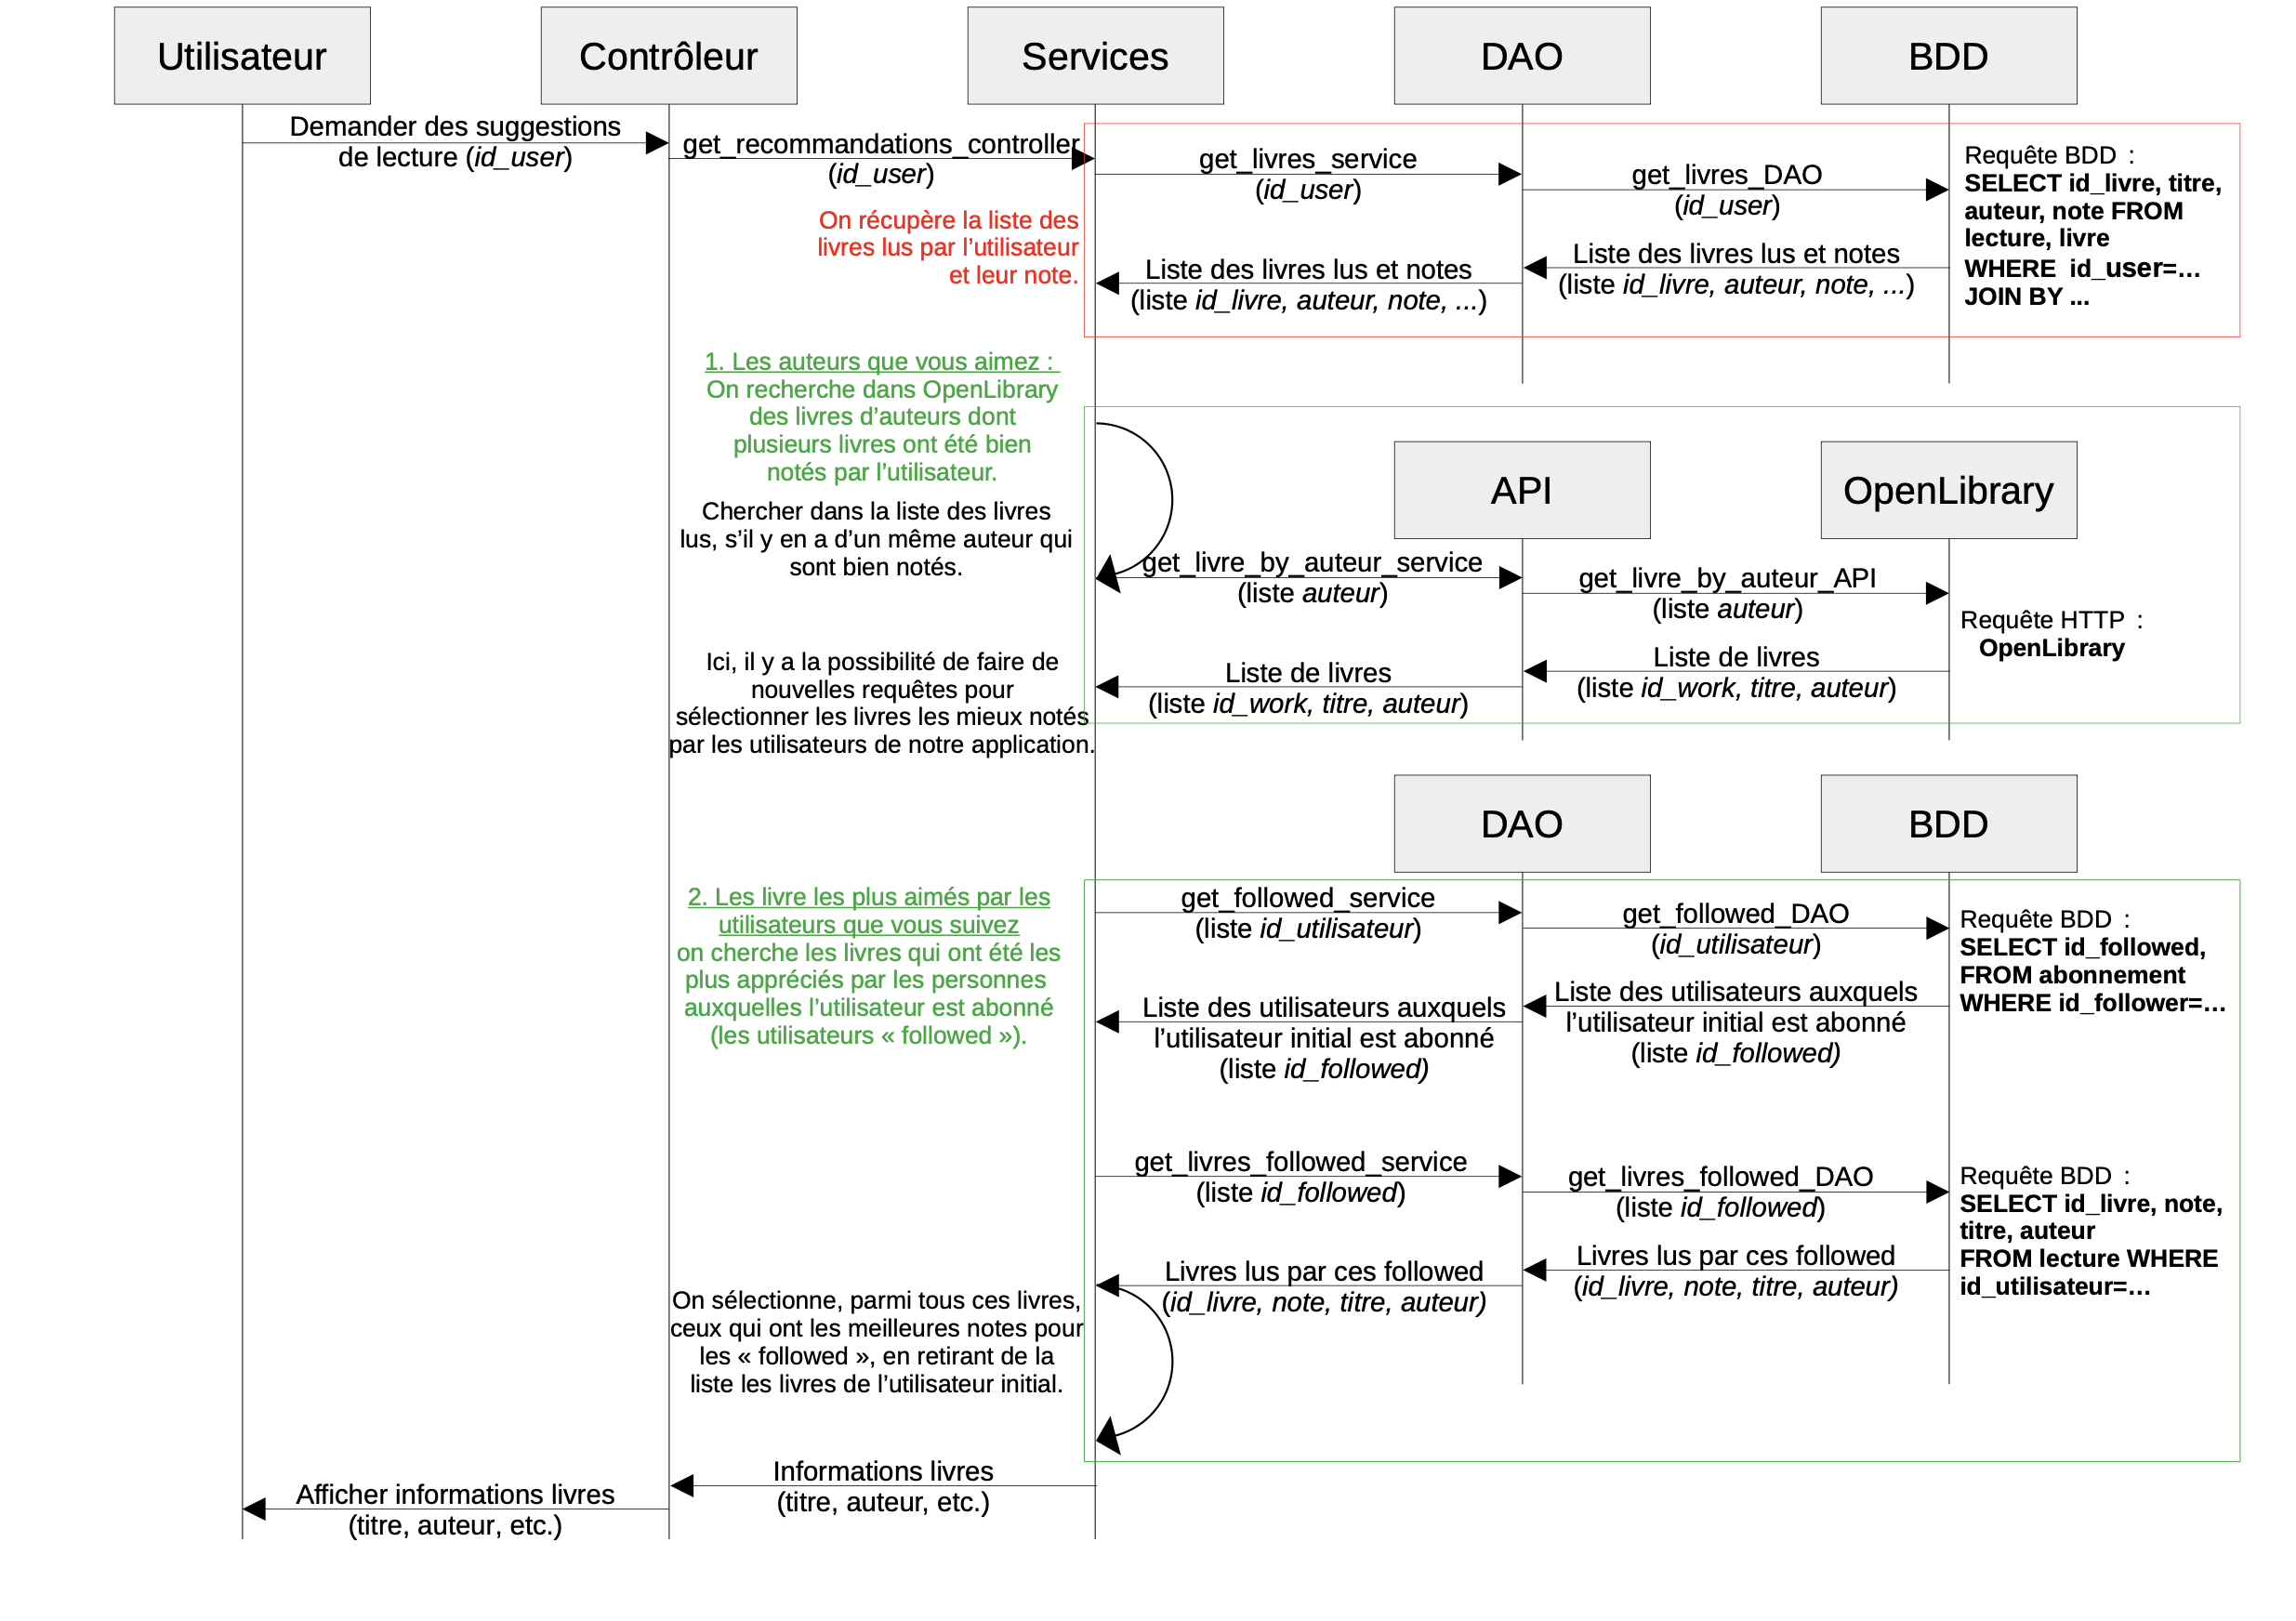
\includegraphics[width=0.8\textwidth]{Diagramme_Séquence_demander-des-recommandations_page-0001.jpg}

Figure 11 – Diagramme de séquence : demander des recommandations
\end{center}

Le but de cette séquence est de recommander à l'utilisateur des livres
qu'il n'a pas enregistrés et qui seraient susceptibles de lui plaire.

Il se situe sur sa page d'accueil, et clique sur un bouton «
Recommandations personnelles ».

La première étape est de récupérer la liste des livres lus par cet
utilisateur (\texttt{id\_livre}), ainsi que les notes associées à chacun
de ces livres (\texttt{note}). On se sert pour cela de la table
\texttt{lecture}, qui enregistre les lectures d'un utilisateur.

Nous envisageons ensuite plusieurs possibilités pour effectuer des
recommandations.

\ul{Premier type de recommandations : ``Les auteurs que vous aimez''}

Si dans les livres lus par l'utilisateur, plusieurs livres d'un même
auteur sont bien notés, d'autres livres du même auteur lui seront
proposés.

Le \textbf{Service} va donc essayer d'identifier dans la liste de livres
de l'utilisateur les auteurs les plus appréciés. S'il trouve des
candidats, il va interroger \textbf{OpenLibrary}, via l'\textbf{API},
pour rechercher d'autres livres des mêmes auteurs.

Il est également possible de rechercher, parmi ces livres d'auteurs
appréciés par l'utilisateur, ceux qui ont les meilleures notes dans
notre application Ex-Libris, mais cela n'apparaît que comme commentaire
sur le diagramme de séquence pour ne pas alourdir le schéma.

\ul{Deuxième type de recommandations : ``Les livres les plus aimés par
les utilisateurs que vous suivez''}

Cette fois-ci, nous allons utiliser la fonctionnalité d'abonnement pour
offrir des recommandations à l'utilisateur.

Dans un premier temps, il s'agira de récupérer la liste des utilisateurs
auxquels celui-ci est abonné (\texttt{id\_followed} dans la table
\texttt{Abonnement}).

Ensuite, l'application cherchera, dans les lectures de ces ``followed'',
les livres les mieux notés, et les proposera à l'utilisateur.

À la fin de l'exécution des algorithmes de recommandations au niveau du
\textbf{Service}, celui-ci va transmettre au \textbf{Contrôleur} une
liste des livres recommandés pour l'utilisateur (\texttt{titre},
\texttt{auteur}, etc.), que ce dernier va mettre en forme et afficher
pour l'utilisateur.

\ul{Autres types de recommandations (en projet) :}

Nous venons de présenter 2 méthodes de recommandation, à titre
d'illustration, mais nous avons le projet d'en développer d'autres.

En effet, les recommandations précédentes nécessitent des conditions
(avoir noté plusieurs livres d'un même auteur pour la première, avoir
des abonnements pour la seconde). Nous envisageons de faire des
recommandations du type : ``les livres les mieux notés'' ou ``les livres
suscitant le plus de critiques''.

Nous avons conscience que ``les livres les mieux notés'' peut susciter
des requêtes assez lourdes, nous avons donc envisagé la possibilité
d'ajouter un champ \texttt{note\_moyenne} à la table \texttt{livre}, qui
pourrait être mis à jour à chaque nouvelle note sur un livre.

Un autre type d'algorithme envisagé serait de recouper les livres lus et
bien notés entre l'utilisateur initial et d'autres utilisateurs de
l'application. Nous obtiendrions alors des utilisateurs avec des goûts
similaires à l'utilisateur initial.

Ainsi, en prenant les livres bien notés de ces utilisateurs avec des
goûts similaires, nous pourrions alors faire de nouvelles suggestions à
l'utilisateur.

Encore une fois, nous avons conscience de la charge potentielle de
telles requêtes, et réflechissons aux possibilités pour les alléger.

\newpage

partie 1 : Cahier des Charges partie 2 : Maquette de l'application

📋 Suivi projet Ex-Libris

✅ Fait

\begin{itemize}
\tightlist
\item
  Arno : diagramme de séquence (partie 2)
\item
  Paul : diagramme de Gantt (partie 1)
\item
  Paul : présentation de l'API (partie 1)
\item
  Paul : répartition des tâches (partie 1)
\item
  Cecile : Diagramme de cas d'utilisation (partie 1)
\end{itemize}

🔄 En cours

\begin{itemize}
\tightlist
\item
  Moussa : diagramme BDD (partie 2)
\item
  Axel : diagramme d'activité (partie 1)
\item
  Anne-Camille : diagramme de classe business (détail + explication des
  classes) (partie 2)
\item
  Paul : Introduction
\end{itemize}

⬜ À faire

\begin{itemize}
\tightlist
\item
  Partie répartition des tâches et présentation de l'équipe (partie 2)
\item
  Diagramme de package (DAO / Services / Business / View) (partie 2)
\item
  Détail d'un service (partie 2)
\item
  Présentation de l'API (partie 1) \ldots{}
\end{itemize}




\end{document}
